\documentclass[border=0pt]{standalone}

\def\xcolorversion{2.00}

\usepackage[utf8]{inputenc} 


\usepackage{tikz}
\usetikzlibrary{arrows,%
                shapes,positioning,
                decorations.text,decorations.pathreplacing}
                
\thispagestyle{empty}
\begin{document}

  
%\begin{center}
%\hspace{-2cm}
\begin{tikzpicture}[node distance   = 1.5 cm]
\centering
  %\useasboundingbox (-1,-1) rectangle (11,11); 
  \tikzset{VertexStyle/.style = {shape          = circle,
                                 ball color     = yellow,
                                 text           = black,
                                 inner sep      = 2pt,
                                 outer sep      = 0pt,
                                 minimum size   = 24 pt}}
  \tikzset{EdgeStyle/.style   = {thick,
                                 double          = yellow,
                                 double distance = 1pt}}
  \tikzset{LabelStyle/.style =   {draw,
                                  fill           = yellow,
                                  text           = red}}
     % n=0
     \node[VertexStyle](A){$B_{-1}$};
     % n=1
     \node[VertexStyle, below left=of A](B1){$B_{00}$};
     \draw[EdgeStyle](A) to node{} (B1) ;
     \node[VertexStyle, below right=of A](B2){$B_{01}$};
     \draw[EdgeStyle, double=red, double distance=3pt](A) to node{} (B2);
     % n=2
     \node[VertexStyle, below=of B1](C1){$B_{10}$};
     \draw[EdgeStyle](C1) to node{} (B1); 
     \node[VertexStyle, below=of B2](C2){$B_{11}$};
     \draw[EdgeStyle, bend left=20](C2) to node{} (B1); 
     \draw[EdgeStyle](C2) to node{} (B1); 
     \draw[EdgeStyle, bend right=20](C2) to node{} (B1); 
     %\draw[EdgeStyle, bend left=20](C2) to node{} (B1); 
     \draw[EdgeStyle, double=red, double distance=3pt](C2) to node{} (B2); 
     % n=3
     \node[VertexStyle, below=of C1](D1){$B_{20}$};
     \draw[EdgeStyle](D1) to node{} (C1); 
     \node[VertexStyle, below=of C2](D2){$B_{21}$};
     \draw[EdgeStyle, bend right=14, double=red, double distance=3pt](D1) to node{} (C2); 
     \draw[EdgeStyle, bend left=14](D1) to node{} (C2); 
     \draw[EdgeStyle](D2) to node{} (C2); 


%%% CUTTING STACKING 0 %%%
\node[right=of A](cs0)
{
\begin{tikzpicture}
  \tikzset{VertexStyle/.style = {shape          = circle,
                                 ball color     = yellow,
                                 text           = black,
                                 inner sep      = 2pt,
                                 outer sep      = 0pt,
                                 minimum size   = 24 pt}}
    \begin{scope}[every label/.style={inner sep=5pt, draw=none,rectangle,fill=none}, every node/.style={fill=black,circle,inner sep=0pt,minimum size=5pt}, blabel/.style={label={above:#1}}, bblabel/.style 2 args={label={[label distance=#2, VertexStyle]below:#1}}, alabel/.style={label={above:#1}}]
	%%% TOUR DE GAUCHE %%%
    \tikzset{node distance = 3 cm}
	\node[blabel={$0$}{}](a){};
	\node[right=of a, blabel={$1$}](b){};
	\draw(a) to node[bblabel={$B_{-1}$}{0pt}, draw=none, fill=none]{} (b) ;
	\node[right=2.7cm of a, label={[blue, inner sep=3pt]above:$x$}, fill=blue](x){};
  \end{scope}
\end{tikzpicture}
};


%%% CUTTING STACKING 1 %%%
%\node[left=of B1](cs1)
\node (cs1) at ([shift=({-100pt,20pt})]B1)
{
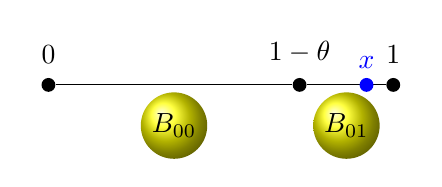
\begin{tikzpicture}
  \tikzset{VertexStyle/.style = {shape          = circle,
                                 ball color     = yellow,
                                 text           = black,
                                 inner sep      = 2pt,
                                 outer sep      = 0pt,
                                 minimum size   = 24 pt}}
    \begin{scope}[every label/.style={inner sep=5pt, draw=none,rectangle,fill=none}, every node/.style={fill=black,circle,inner sep=0pt,minimum size=5pt}, blabel/.style={label={above:#1}}, bblabel/.style 2 args={label={[label distance=#2, VertexStyle]below:#1}}, alabel/.style={label={above:#1}}]
	%%% TOUR DE GAUCHE %%%
    \tikzset{node distance = 3 cm}
	\node[blabel={$0$}{}](a){};
	\node[right=of a, blabel={$1-\theta$}](b){};
	\draw(a) to node[bblabel={$B_{00}$}{0pt}, draw=none, rectangle, fill=none]{} (b);
	%%% TOUR DE DROITE %%%
	%
	\tikzset{node distance = 1 cm};
	\node[right=of b, blabel={$1$}](c){};
	%
	\draw(b) to node[bblabel={$B_{01}$}{0pt}, draw=none, rectangle, fill=none]{} (c);
	\node[left=0.15cm of c, label={[blue, inner sep=3pt]above:$x$}, fill=blue](x){};
  \end{scope}
\end{tikzpicture}
};

%%% CUTTING STACKING 2 %%%
\node[right=0.5cm of C2](cs2)
{
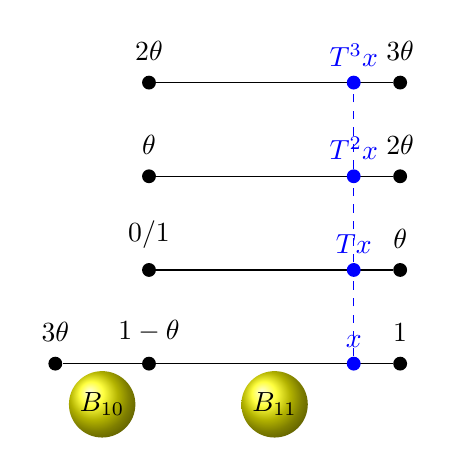
\begin{tikzpicture}
  \tikzset{VertexStyle/.style = {shape          = circle,
                                 ball color     = yellow,
                                 text           = black,
                                 inner sep      = 2pt,
                                 outer sep      = 0pt,
                                 minimum size   = 24 pt}}
    \begin{scope}[every label/.style={inner sep=5pt, draw=none,rectangle,fill=none}, every node/.style={fill=black,circle,inner sep=0pt,minimum size=5pt}, bblabel/.style 2 args={label={[label distance=#2, VertexStyle]below:#1}}, blabel/.style={label={above:#1}}]
	%%% TOUR DE GAUCHE %%%
    \tikzset{node distance = 1 cm}
	\node[blabel={$3\theta$}{}](a){};
	\node[right=of a, blabel={$1-\theta$}](b){};
	\draw(a) to node[bblabel={$B_{10}$}{0pt}, draw=none, rectangle, fill=none]{} (b);
	%%% TOUR DE DROITE %%%
	%
	\tikzset{node distance = 1 cm};
	\node[above=of b, blabel={$0/1$}](b1){};
	\node[above=of b1, blabel={$\theta$}](b2){};
	\node[above=of b2, blabel={$2\theta$}](b3){};
	%
	\tikzset{node distance = 3 cm};
	\node[right=of b, blabel={$1$}](c){};
	%
	\tikzset{node distance = 1 cm};
	\node[above=of c, blabel={$\theta$}](c1){};
	\node[above=of c1, blabel={$2\theta$}](c2){};
	\node[above=of c2, blabel={$3\theta$}](c3){};
	\draw(b) to node[bblabel={$B_{11}$}{0pt}, draw=none, rectangle, fill=none]{} (c);
	\draw(b1) to (c1);
	\draw(b2) to (c2);
	\draw(b3) to (c3);
	%%% CLASSE DE x %%%
	%
	\node[distance=0.5cm, left=0.4cm of c, fill=blue, label={[blue, inner sep=3pt]above:$x$}](x){};
	%
	\node[above=of x, label={[blue, inner sep=3pt]above:$Tx$}, fill=blue](x1){};
	\node[above=of x1, label={[blue, inner sep=3pt]above:$T^2x$}, fill=blue](x2){};
	\node[above=of x2, label={[blue, inner sep=3pt]above:$T^3x$}, fill=blue](x3){};
	\draw[blue, dashed](x) to (x1);
	\draw[blue, dashed](x1) to (x2);
	\draw[blue, dashed](x2) to (x3);
	
  \end{scope}
\end{tikzpicture}
};

%%% CUTTING STACKING 3 %%%
%\node[below=-20pt of cs1](cs3)
\node (cs3) at ([shift=({30pt,-160pt})]cs1)
{
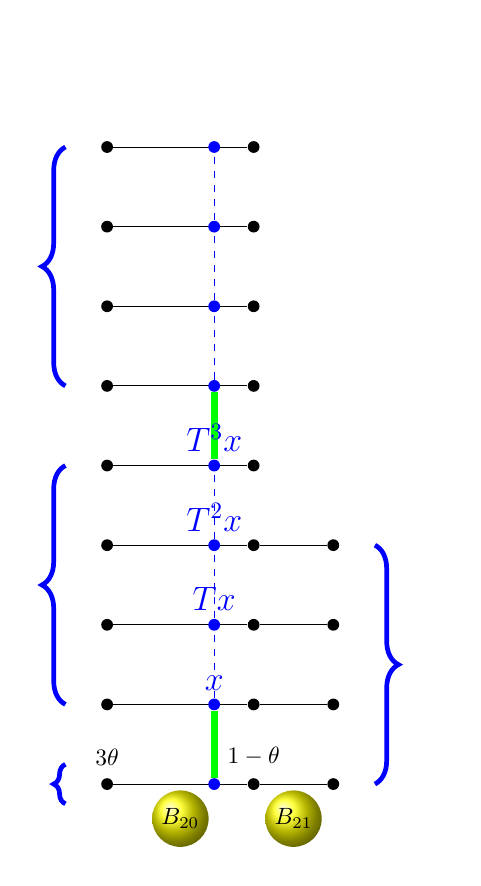
\begin{tikzpicture}
  \tikzset{VertexStyle/.style = {shape          = circle,
                                 ball color     = yellow,
                                 text           = black,
                                 inner sep      = 2pt,
                                 outer sep      = 0pt,
                                 minimum size   = 24 pt}}
	\scalebox{0.85}{
  \begin{scope}[every label/.style={inner sep=5pt, draw=none,rectangle,fill=none}, every node/.style={fill=black,circle,inner sep=0pt,minimum size=5pt}, bblabel/.style 2 args={label={[label distance=#2, VertexStyle]below:#1}}, blabel/.style={label={above:#1}}]
	%%% TOUR DE GAUCHE %%%
    \tikzset{node distance = 2 cm}
	\node[blabel={$3\theta$}{}](a){};
	\node[right=of a, blabel={$1-\theta$}](b){};
	\draw(a) to node[bblabel={$B_{20}$}{0pt}, draw=none, rectangle, fill=none]{} (b);
	\tikzset{node distance = 1 cm}
	\node[above=of a](a1){};
	\node[above=of a1](a2){};
	\node[above=of a2](a3){};	
	\node[above=of a3](a4){};
	\node[above=of a4](a5){};
	\node[above=of a5](a6){};
	\node[above=of a6](a7){};
	\node[above=of a7](a8){};
	\node[above=of b](b1){};
	\node[above=of b1](b2){};
	\node[above=of b2](b3){};
	\node[above=of b3](b4){};
	\node[above=of b4](b5){};
	\node[above=of b5](b6){};
	\node[above=of b6](b7){};
	\node[above=of b7](b8){};
	\draw(a1) to (b1);
	\draw(a2) to (b2);
	\draw(a3) to (b3);
	\draw(a4) to (b4);
	\draw(a5) to (b5);
	\draw(a6) to (b6);
	\draw(a7) to (b7);
	\draw(a8) to (b8);
	%%% TOUR DE DROITE %%%
	%
	\tikzset{node distance = 1 cm};
	\node[right=of b](c){};
	\node[right=of b1](c1){};
	\node[right=of b2](c2){};
	\node[right=of b3](c3){};
	\draw(b) to node[bblabel={$B_{21}$}{0pt}, draw=none, rectangle, fill=none]{} (c);
	\draw(b1) to (c1);
	\draw(b2) to (c2);
	\draw(b3) to (c3);
	%%% ORBITE %%%
	\node[distance=0.25cm, left=0.4cm of b, fill=blue](x){};
	\tikzset{node distance = 1 cm};
	\node[above=of x, fill=blue, label={[blue, inner sep=3pt]above:{\Large $x$}}](x1){};
	\node[above=of x1, fill=blue, label={[blue, inner sep=3pt]above:\Large $Tx$}](x2){};
	\node[above=of x2, fill=blue, label={[blue, inner sep=3pt]above:\Large $T^2x$}](x3){};	
%	\node[above=of x3, fill=blue, label={[blue, inner sep=3pt]above:\Large $T^3x$}](x4){};
	\node[above=of x3, draw=none, fill=none](x4){};
	\node[above=of x4, fill=blue](x5){};
	\node[above=of x5, fill=blue](x6){};
	\node[above=of x6, fill=blue](x7){};
	\node[above=of x7, fill=blue](x8){};
	\draw[green, line width=1mm](x) to (x1);
	\draw[blue, dashed](x1) to (x2);
	\draw[blue, dashed](x2) to (x3);
	\draw[blue, dashed](x3) to (x4);
	\draw[green, line width=1mm](x4) to (x5);
	\node[above=of x3, fill=blue, label={[blue, inner sep=3pt]above:\Large $T^3x$}](xx4){};
	\draw[blue, dashed](x5) to (x6);
	\draw[blue, dashed](x6) to (x7);
	\draw[blue, dashed](x7) to (x8);
	%% BRACES %%
	\draw[decorate, decoration={brace,amplitude=10pt, raise=15pt}, blue, line width=2pt] (a1.west) -- (a4.west);
	\draw[decorate, decoration={brace,amplitude=10pt, raise=15pt}, blue, line width=2pt] (a5.west) -- (a8.west);
	\node[node distance=3pt, above=of a, fill=none](ashiftdown){};
	\node[node distance=3pt, below=of a, fill=none](ashiftup){};
	\draw[decorate, decoration={brace,amplitude=5pt, raise=15pt}, blue, line width=2pt] (ashiftup.west)--(ashiftdown.west);
	\draw[decorate, decoration={brace,amplitude=10pt, raise=15pt, mirror}, blue, line width=2pt] (c.east) -- (c3.east);
  \end{scope}
}
\end{tikzpicture}
};

  \end{tikzpicture}
%\end{center}
\end{document}